\section{整体观测与导数观测}
\label{sec:opt-fit-global}

到目前为止，读数都是有限个数。另一类常见任务是：整个区域上都有一份带误差的函数值，例如一幅含噪图像或一条连续记录的信号，要找一个更“规则”的函数贴近它；或者手里有的不是函数值，而是一个梯度场，例如由相邻像素差估计出的斜率，要找一个梯度最接近它的函数。这时观测不再是有限个泛函，表示定理不能直接使用。本节用两种几何工具求解：函数值观测在核积分算子的谱坐标中逐方向配方，梯度观测则化为到一个闭子空间的投影。它们都只用到二次目标的配方和Hilbert空间的投影，不需要下一章才建立的泛函微分。

\subsection{函数值观测下的拟合}
\label{sec:opt-fit-function-values}

\paragraph{两个空间与目标}
设$X$是紧度量空间，$\nu$是$X$上全支撑的有限正Borel测度，$K$是$X\times X$上连续的半正定核，$H=H_K$是它的再生核Hilbert空间。数据是$y\in L^2(\nu)$，它只是一个平方可积的等价类，不必属于$H$；候选$f$则取自$H$。由$|f(x)|\le\sqrt{K(x,x)}\,\|f\|_H$，
\[
  \|f\|_{L^2(\nu)}^2\le\Bigl(\sup_xK(x,x)\Bigr)\nu(X)\,\|f\|_H^2,
\]
所以把$f$看作$L^2(\nu)$的元素是一个有界的线性嵌入。于是对$\lambda>0$可以定义目标
\begin{equation}
  J(f)=\|f-y\|_{L^2(\nu)}^2+\lambda\|f\|_H^2,\qquad f\in H .
  \label{eq:opt-fit-global-objective}
\end{equation}
第一项在$L^2$中度量误差，第二项在$H$中度量规则程度，两个范数属于不同的空间。

\paragraph{谱坐标}
求解要用到核积分算子$(T_Kg)(x)=\int_XK(x,z)g(z)\,\mathrm d\nu(z)$的谱。它是$L^2(\nu)$上的紧自伴半正定算子，紧自伴算子的谱定理可参考\BookChapterRef{chap:operator-spectra-equations}{卷二“算子谱与算子方程”章}。按卷二“再生核Hilbert空间”章中的Mercer定理，在上述条件下，$T_K$的正特征值$\mu_1\ge\mu_2\ge\cdots>0$（那里记作$\lambda_j$，本章$\lambda$留给正则化参数）对应$L^2(\nu)$中标准正交的连续特征函数$\psi_j$，$\sum_j\mu_j=\int_XK(x,x)\,\mathrm d\nu(x)<\infty$；而且$f\in H$当且仅当$f=\sum_jb_j\psi_j$且$\sum_jb_j^2/\mu_j<\infty$，此时
\begin{equation}
  \|f\|_{L^2(\nu)}^2=\sum_jb_j^2,\qquad \|f\|_H^2=\sum_j\frac{b_j^2}{\mu_j}.
  \label{eq:opt-fit-spectral-norms}
\end{equation}
$L^2(\nu)$是正谱特征函数张成的闭子空间与零空间$\ker T_K$的正交和。把数据相应地分解为
\[
  y=\sum_jc_j\psi_j+y_0,\qquad c_j=\langle y,\psi_j\rangle_{L^2(\nu)},\quad y_0\in\ker T_K .
\]
$H$中的函数作为$L^2$元素没有零谱分量，所以$y_0$是任何候选都无法贴近的部分。

\paragraph{逐方向配方}
把$f=\sum_jb_j\psi_j$代入目标。由正交分解与式~\eqref{eq:opt-fit-spectral-norms}，
\[
  J(f)=\|y_0\|_{L^2}^2+\sum_j\Bigl[(b_j-c_j)^2+\frac\lambda{\mu_j}b_j^2\Bigr].
\]
每个方括号只含一个坐标，单独配方：
\[
  (b-c)^2+\frac\lambda\mu b^2=\Bigl(1+\frac\lambda\mu\Bigr)\Bigl(b-\frac{\mu c}{\mu+\lambda}\Bigr)^2+\frac{\lambda c^2}{\mu+\lambda}.
\]

\begin{theorem}[整体函数值观测下的正则化拟合]
\label{thm:opt-fit-global-values}
在上述设定下，目标~\eqref{eq:opt-fit-global-objective}在$H$上有唯一的最小点
\begin{equation}
  f_\lambda=\sum_jb_j^\star\psi_j,\qquad b_j^\star=\frac{\mu_j}{\mu_j+\lambda}c_j ,
  \label{eq:opt-fit-spectral-solution}
\end{equation}
最小值为$\|y_0\|_{L^2}^2+\sum_j\lambda c_j^2/(\mu_j+\lambda)$。
\end{theorem}

\begin{proof}
先核验$f_\lambda$确实属于$H$。由$\mu/(\mu+\lambda)^2\le1/(4\lambda)$（对$\mu>0$，等号在$\mu=\lambda$），$\sum_j(b_j^\star)^2/\mu_j=\sum_j\mu_jc_j^2/(\mu_j+\lambda)^2\le\sum_jc_j^2/(4\lambda)\le\|y\|_{L^2}^2/(4\lambda)<\infty$。再比较任一$f=\sum_jb_j\psi_j\in H$：由上面的配方，各项都是非负数之和，级数可以逐项相减，
\[
  J(f)-J(f_\lambda)=\sum_j\Bigl(1+\frac\lambda{\mu_j}\Bigr)(b_j-b_j^\star)^2\ge0,
\]
等号当且仅当每个$b_j=b_j^\star$，即$f=f_\lambda$。最小值由配方的余项求和得到。
\end{proof}

注意$\sum_jc_j^2$只等于正谱部分的范数平方$\|y-y_0\|_{L^2}^2$，不是$\|y\|_{L^2}^2$；漏掉$y_0$会低估不可消除的误差。

\paragraph{一个可以对照闭式的例子}
在$[0,1]$上取最小值核与Lebesgue测度。卷二“再生核Hilbert空间”章已算出$\mu_j=\omega_j^{-2}$、$\psi_j=\sqrt2\sin\omega_jx$，$\omega_j=(j-\tfrac12)\pi$，零空间平凡。取数据$y=1$，它不属于$H_{\min}$（后者要求$f(0)=0$），谱坐标为$c_j=\int_0^1\sqrt2\sin\omega_jx\,\mathrm dx=\sqrt2/\omega_j$。由式~\eqref{eq:opt-fit-spectral-solution}，$f_\lambda=\sum_j\frac{\sqrt2}{\omega_j(1+\lambda\omega_j^2)}\sqrt2\sin\omega_jx$。把级数求和，它与函数$1-\cosh\bigl((1-x)/\sqrt\lambda\bigr)/\cosh(1/\sqrt\lambda)$一致（例如$\lambda=0.1$时，两者在$x=\tfrac12$处都约为$0.786$）；这个闭式在下一章可以由变分条件直接得到。图~\ref{fig:opt-fit-spectral-shrinkage}(b)画出了三个$\lambda$下的拟合：函数被迫从$f(0)=0$出发，在宽度约为$\sqrt\lambda$的边界层内升到接近$1$，然后与数据贴合。$\lambda$越小，边界层越窄。

\begin{figure}[!htbp]
  \centering
  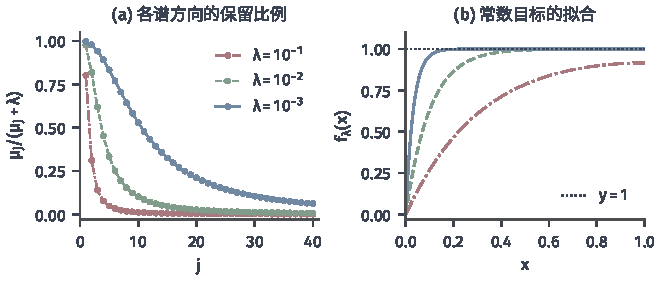
\includegraphics[width=112mm]{figures/03-optimization-evolution-and-signals/01-optimization/matplotlib/c8-spectral-shrinkage/figure.pdf}
  \caption{整体观测下的谱收缩，最小值核、$[0,1]$上Lebesgue测度，$\mu_j=((j-\tfrac12)\pi)^{-2}$。(a)~前$40$个谱方向的保留比例$\mu_j/(\mu_j+\lambda)$，$\lambda=10^{-1},10^{-2},10^{-3}$：比例随$j$平滑下降，没有在某个序号处截断。(b)~常数数据$y=1$（黑色点线）的拟合$f_\lambda$，线型与(a)对应；由于$H_{\min}$中的函数在$0$处为零，拟合在宽度约$\sqrt\lambda$的边界层内升起。三个$\lambda$下的有效维度$\sum_j\mu_j/(\mu_j+\lambda)$依次约为$1.58$、$5.00$、$15.81$。}
  \label{fig:opt-fit-spectral-shrinkage}
\end{figure}

\paragraph{正则化重新分配谱权重}
式~\eqref{eq:opt-fit-spectral-solution}说明，正则化对每个谱方向乘以因子$\mu_j/(\mu_j+\lambda)$。$\mu_j\gg\lambda$的方向几乎原样保留，$\mu_j\ll\lambda$的方向被压缩为原来的约$\mu_j/\lambda$。图~\ref{fig:opt-fit-spectral-shrinkage}(a)显示，因子随$j$平滑下降，并不在某个序号处由$1$突然变为$0$：正则化改变的是整个候选的频谱权重，而不是删去序号超过某个阈值的所有方向。这与第~\ref{sec:opt-fit-linear-basis}小节的岭回归滤波$\sigma_k^2/(\sigma_k^2+\lambda)$是同一种机制。有限个点值观测时也是如此：拟合读数$\bm G\bm a_\lambda=\bm G(\bm G+n\lambda\bm I)^{-1}\bm y$在$\bm G$的第$k$个特征方向上乘以$t_k/(t_k+n\lambda)$，$t_k$是Gram矩阵的特征值。有限Gram矩阵只有$n$个特征值，整体算子有无限多个；两者怎样随参数和数据变化，留到第~\ref{sec:opt-fit-error}节统一讨论。

\paragraph{有效维度}
把这些因子加起来，
\[
  N(\lambda)=\sum_j\frac{\mu_j}{\mu_j+\lambda},
\]
可以理解为在正则尺度$\lambda$下“有效保留”的谱方向个数：完全保留的方向计$1$，完全压掉的方向计$0$，部分保留的计其比例。称$N(\lambda)$为\term{有效维度}（effective dimension）。由于每项不超过$\mu_j/\lambda$，而Mercer定理保证$\sum_j\mu_j<\infty$（$T_K$是迹类算子），$N(\lambda)\le\lambda^{-1}\sum_j\mu_j<\infty$；即使谱方向有无限多个，有效维度也是有限数。对上面的最小值核，$\sum_j\mu_j=\tfrac12$，$\lambda=10^{-1},10^{-2},10^{-3}$时$N(\lambda)$约为$1.58$、$5.00$、$15.81$，大致按$1/(2\sqrt\lambda)$增长，远小于粗略上界$1/(2\lambda)$。

有效维度是给定核、测度与正则参数下的确定性量。它不是函数类的覆盖数，也不是实际计算时使用的特征个数；整体观测下的这个确定性结论，也不能自动变成有限随机样本下的泛化保证。

\subsection{导数观测下的拟合}
\label{sec:opt-fit-gradient-observations}

\paragraph{问题}
设$\Omega\subset\mathbb R^d$是有界连通的Lipschitz区域，给定向量场$\bm v\in L^2(\Omega;\mathbb R^d)$，以及一个$g\in H^1(\Omega)$，用它的边界迹规定边界值。要在边界值固定的函数中找梯度最接近$\bm v$的一个：
\begin{equation}
  \min_{u\in g+H_0^1(\Omega)}\ \frac12\|\nabla u-\bm v\|_{L^2(\Omega)}^2 .
  \label{eq:opt-fit-gradient-problem}
\end{equation}
这里用到的弱导数、Sobolev空间$H^1$与$H_0^1$、边界迹以及Poincaré不等式，可参考\BookChapterRef{chap:weak-derivatives-sobolev}{卷二“弱导数与Sobolev空间”章}。需要的结论是：存在常数$C_\Omega$，使所有$w\in H_0^1(\Omega)$满足$\|w\|_{L^2}\le C_\Omega\|\nabla w\|_{L^2}$。

\paragraph{化为投影}
令$u=g+w$，$w\in H_0^1(\Omega)$，目标变成$\tfrac12\|\nabla w-(\bm v-\nabla g)\|_{L^2}^2$。记
\[
  V=\{\nabla w:w\in H_0^1(\Omega)\}\subseteq L^2(\Omega;\mathbb R^d),
\]
问题就是求$\bm v-\nabla g$到$V$的最近点。$V$是线性子空间；要用投影定理，还需要它是闭的。

\begin{lemma}[梯度像是闭子空间]
\label{lem:opt-fit-gradient-closed}
$V$在$L^2(\Omega;\mathbb R^d)$中闭，且映射$w\mapsto\nabla w$在$H_0^1(\Omega)$上单射。
\end{lemma}

\begin{proof}
设$w_k\in H_0^1$，$\nabla w_k\to\bm z$于$L^2$。则$(\nabla w_k)$是Cauchy列。由Poincaré不等式，$\|w_k-w_m\|_{L^2}\le C_\Omega\|\nabla w_k-\nabla w_m\|_{L^2}$，所以$\|w_k-w_m\|_{H^1}^2=\|w_k-w_m\|_{L^2}^2+\|\nabla(w_k-w_m)\|_{L^2}^2\le(1+C_\Omega^2)\|\nabla w_k-\nabla w_m\|_{L^2}^2$，$(w_k)$是$H^1$中的Cauchy列。$H^1$完备，$H_0^1$是它的闭子空间，于是$w_k\to w\in H_0^1$于$H^1$，特别地$\nabla w_k\to\nabla w$于$L^2$。由极限唯一，$\bm z=\nabla w\in V$。单射性：若$\nabla w=\bm 0$，Poincaré不等式给出$\|w\|_{L^2}=0$。
\end{proof}

\begin{theorem}[梯度场拟合]
\label{thm:opt-fit-gradient}
问题~\eqref{eq:opt-fit-gradient-problem}有唯一解$u^\star=g+w^\star$，其中$\nabla w^\star$是$\bm v-\nabla g$在$V$上的正交投影。解由正交条件刻画：
\begin{equation}
  \int_\Omega(\nabla u^\star-\bm v)\cdot\nabla h\,\mathrm dx=0\qquad\text{对一切}\ h\in H_0^1(\Omega).
  \label{eq:opt-fit-gradient-orthogonality}
\end{equation}
\end{theorem}

\begin{proof}
由引理~\ref{lem:opt-fit-gradient-closed}，$V$是Hilbert空间$L^2(\Omega;\mathbb R^d)$的闭子空间，投影定理给出唯一的最近点$\bm z^\star\in V$，它由$\bm v-\nabla g-\bm z^\star\perp V$刻画。再由单射性，$\bm z^\star=\nabla w^\star$中的$w^\star\in H_0^1$唯一。$u\in g+H_0^1$与$w=u-g$一一对应，目标值相同，所以$u^\star=g+w^\star$是唯一解。正交条件$\langle\bm v-\nabla g-\nabla w^\star,\nabla h\rangle_{L^2}=0$对一切$h\in H_0^1$成立，即式~\eqref{eq:opt-fit-gradient-orthogonality}。
\end{proof}

推导中没有对$u$求任何泛函导数，也不要求$\bm v$恰好是某个函数的梯度；数据场中不是梯度的部分，就留在与$V$正交的余项里。

\paragraph{一维与二维的例子}
在$\Omega=(0,1)$上取$g=0$，即要求$u(0)=u(1)=0$。此时$V=\{w':w\in H_0^1(0,1)\}$恰是均值为零的$L^2$函数：$w(1)-w(0)=\int_0^1w'=0$；反过来，任一零均值的$z\in L^2$的原函数$\int_0^xz$属于$H_0^1$。到零均值子空间的投影就是减去均值，所以$(u^\star)'=v-\int_0^1v$。例如$v\equiv1$时$u^\star=0$，余项$v-(u^\star)'=1$与每个$h'$（$h\in H_0^1$）正交，因为$\int_0^1h'=0$：固定的边界值不允许函数整体爬升，常数斜率完全无法被吸收。

二维时，余项可以是“旋转”的。在单位正方形上取$\varphi=\sin\pi x\sin\pi y$（它属于$H_0^1$）与$\psi=0.8\varphi$，令
\[
  \bm v=\nabla\varphi+(\partial_y\psi,\,-\partial_x\psi).
\]
对$h\in C_c^\infty$，分部积分得$\int(\partial_y\psi\,\partial_xh-\partial_x\psi\,\partial_yh)=-\int(\partial_x\partial_y\psi-\partial_y\partial_x\psi)h=0$，再由稠密性推广到一切$h\in H_0^1$。所以第二项与$V$正交，而$\nabla\varphi\in V$，投影恰好是$\nabla\varphi$，$u^\star=\varphi$。图~\ref{fig:opt-fit-gradient-projection}把三个场并排画出：给定场同时有发散与旋转，投影保留了从中心向外的“梯度部分”，余项则是绕中心旋转的场，它不是任何函数的梯度，拟合无法也不应吸收它。

\begin{figure}[!htbp]
  \centering
  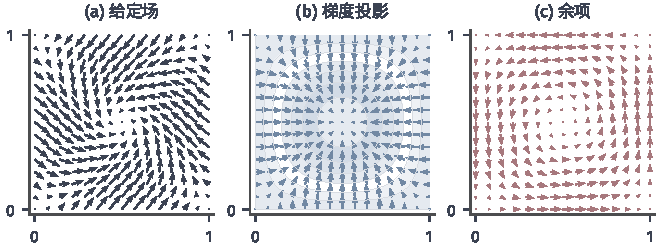
\includegraphics[width=112mm]{figures/03-optimization-evolution-and-signals/01-optimization/matplotlib/c8-gradient-projection/figure.pdf}
  \caption{单位正方形上的梯度场拟合，零边界值。(a)~给定场$\bm v=\nabla\varphi+(\partial_y\psi,-\partial_x\psi)$，$\varphi=\sin\pi x\sin\pi y$，$\psi=0.8\sin\pi x\sin\pi y$；(b)~它在$V=\{\nabla w:w\in H_0^1\}$上的投影$\nabla u^\star=\nabla\varphi$，底色为$u^\star=\varphi$的等值区域；(c)~余项$\bm v-\nabla u^\star=(\partial_y\psi,-\partial_x\psi)$，它与$V$正交，是绕中心旋转的场。箭头长度按同一比例缩放。}
  \label{fig:opt-fit-gradient-projection}
\end{figure}

\paragraph{自由边界}
若不规定边界值，在整个$H^1(\Omega)$中极小化$\tfrac12\|\nabla u-\bm v\|^2$，加任意常数不改变目标，解至多唯一到常数。改在零均值子空间$\{u\in H^1:\int_\Omega u=0\}$中求解，用Poincaré--Wirtinger不等式$\|u-u_\Omega\|_{L^2}\le C\|\nabla u\|_{L^2}$（$u_\Omega$为均值，这里需要$\Omega$连通）代替上面的Poincaré不等式，同样的论证说明梯度像闭、映射单射，于是存在唯一的零均值解，一般解为它加任意常数。在$(0,1)$上，任何$v\in L^2$都是其原函数的导数，于是自由边界的解满足$u'=v$，余项为零，与固定边界的情形形成对照。把正交条件~\eqref{eq:opt-fit-gradient-orthogonality}改写成区域内的方程与边界条件（自由边界时出现自然边界条件），需要分部积分和泛函微分的语言，留给第~\ref{chap:opt-functional}章；那里不再重复建立这个问题的求解理论。
